\documentclass[es,practica]{uah}

\tema{9}
\titulo{Técnicas de acceso al medio}{Lesson title}
%
\begin{document}

\titulacion{Optativa GIEC y GIT}
\departamento{Teoría de la Señal y Comunicaciones}
\asignatura{Comunicaciones Digitales}{}
\curso{2021/2022} 

\maketitle

\section{Técnicas de espectro ensanchado - DS}

El objetivo de esta práctica es hacer una pequeña simulación de un sistema de comunicaciones que utilice como técnica de acceso al medio un sistema CDMA, y en particular técnicas de secuencia directa (DS). 

La idea es muy sencilla. Partiremos de una señal $x(t)$ que contendrá la información a transmitir, de la forma:

\begin{equation}
	x(t) = \sum_{n=-\infty}^{\infty} a_n h_T(t - nT_b)
\end{equation}

donde $a_n = \pm 1$ y $h_T(t)$ es un pulso rectangular de duración $T_b$ (el periodo de bit).

Esta señal se multiplica por una secuencia pseudoaleatoria (en Matlab la podéis generar simplemente con una función \emph{rand}) que se puede escribir como:

\begin{equation}
	c(t) = \sum_{n=-\infty}^{\infty} c_n p(t - nT_c)
\end{equation}

donde $c_n=\pm 1$ y $p(t)$ es un pulso rectangular de duración $T_c$, de forma que $T_c << T_b$, y $T_b = k\cdot T_c$, con $k$ entero. 

En la siguiente figura (extraída de los apuntes) podéis ver de forma gráfica el proceso: 

\begin{figure*}[h!]
	\centering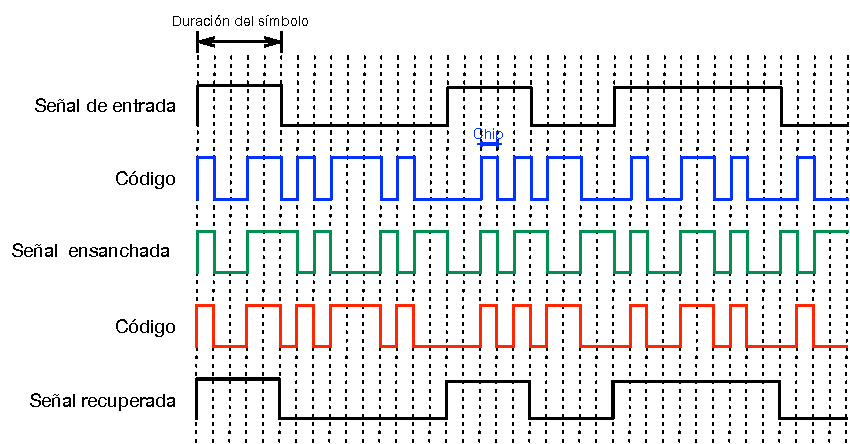
\includegraphics[width=8cm]{./Figuras/DS-CDMA}
\end{figure*}


La señal resultante de multiplicar $x(t)$ por $c(t)$ será nuestra señal de espectro ensanchado. Para recuperar la señal original basta con volver a multiplicar esta señal por el mismo código utilizado en la transmisión. 

A partir de este esquema, realizaremos las siguientes pruebas:

\begin{enumerate}
	\item Generar una señal DS como se ha explicado y comprobar que el sistema funciona correctamente de extremo a extremo, sin interferencias ni ruido. Considerad una duración de la señal suficiente para poder realizar luego las simulaciones con suficiente precisión (e.g. $10^5$ bits)
	\item Añadir una señal interferente (otra señal DS), que simula un segundo usuario en nuestro mismo canal. Comprobar que es posible recuperar el mensaje enviado a partir de la suma de las dos señales DS utilizando el código correcto. Calcular la probabilidad de error de bit para este caso. 
	\item Generar una función que permita visualizar la variación de la probabilidad de error en función de número de interferentes y de la potencia de los mismos. Se debería obtener una figura parecida a la \ref{fig:figura1}, en la que el parámetro $\alpha$ representa la relación entre la señal original y la suma de las interferentes: $y(t) = x(t) + 10^{\alpha/10}\cdot i(t)$.
	

	\begin{figure*}[h!]
		\centering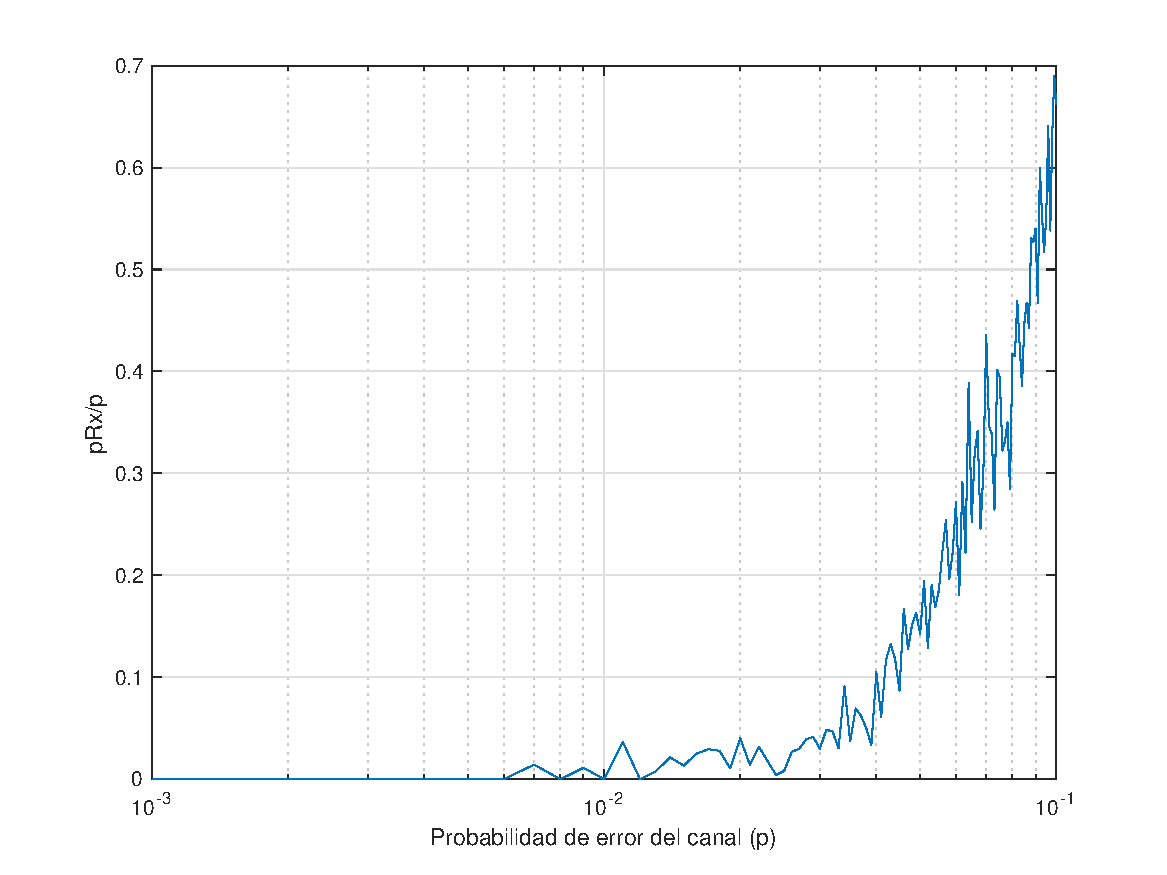
\includegraphics[width=8cm]{./Figuras/Figura1}
		\caption{Salida de ejemplo para el apartado 3}
		\label{fig:figura1}
	\end{figure*}


	\item Comprobar el valor de la probabilidad de error cuando, en ausencia de interferentes, lo que añadimos a nuestra señal original DS es ruido aditivo blanco y gaussiano.
	\item Generar una función que permita visualizar la variación de la probabilidad de error en función de la relación señal a ruido. Como referencia, se debería obtener algo parecido a la figura \ref{fig:figura2}.
	
	\begin{figure*}[h!]
		\centering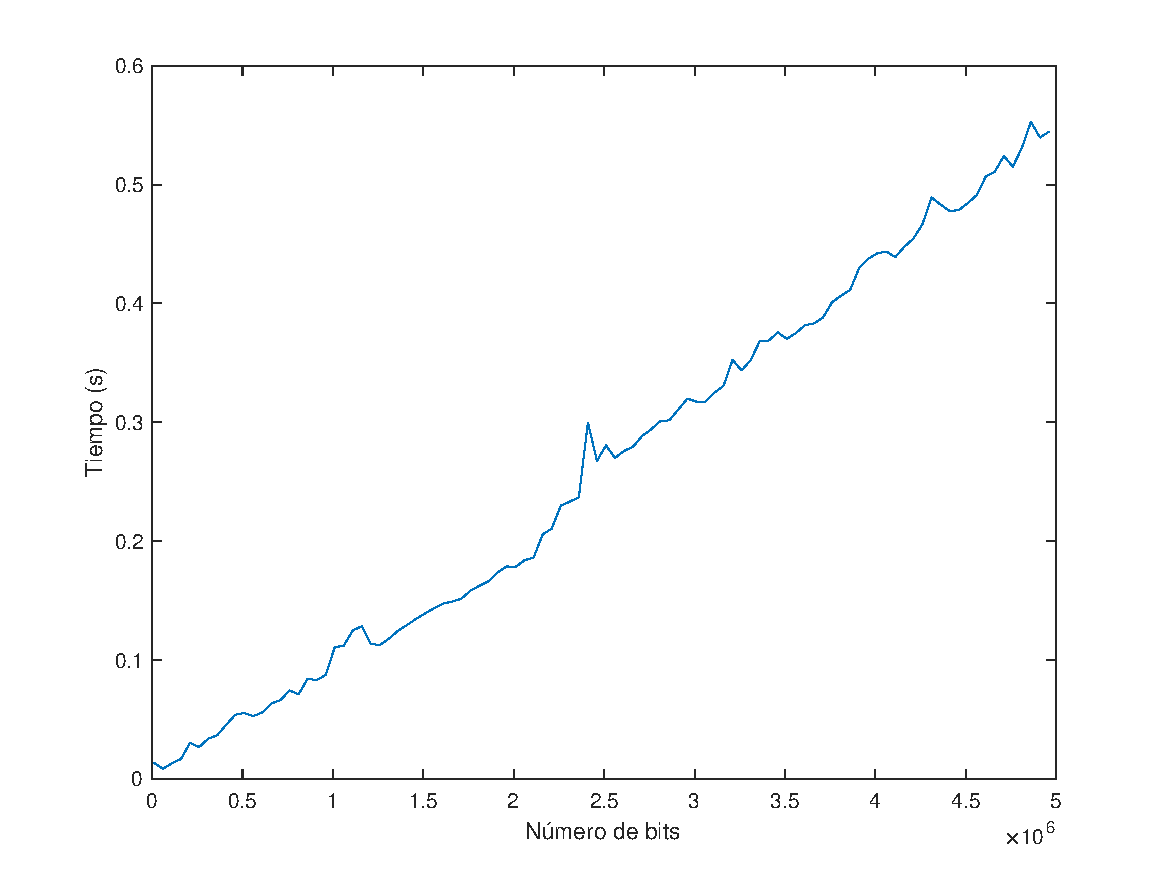
\includegraphics[width=8cm]{./Figuras/Figura2}
		\caption{Salida de ejemplo para el apartado 5}
		\label{fig:figura2}
	\end{figure*}

\end{enumerate}


\section{¿Qué entregar?}
\begin{itemize}
	\item Todas las funciones creadas.
\end{itemize}


%\printindex
\end{document}



	
